\documentclass[10pt, landscape]{article}

\usepackage[a3paper, left=10mm, right=10mm, top=10mm, bottom=10mm]{geometry}
\usepackage{amsmath}
\usepackage{tabularx}
\usepackage{graphicx}
\usepackage{url}
\usepackage{color}
\usepackage{colortbl}

\newcolumntype{L}[1]{>{\raggedright\arraybackslash}p{#1}}
\newcolumntype{C}[1]{>{\centering\arraybackslash}p{#1}}
\newcolumntype{R}[1]{>{\raggedleft\arraybackslash}p{#1}}

\newcolumntype{H}[1]{>{\columncolor{headergray}}c}

\renewcommand{\arraystretch}{2}

\definecolor{headergray}{gray}{0.9}
% Variables
\newcommand*{\mtmiss}{m_\text{miss}^2}
\newcommand*{\EECL}{E_\text{ECL}}
\newcommand*{\costhyl}{\cos\theta_{B, D^{(*)}\ell}}
\newcommand*{\Evis}{E_\text{visible}}

% Arrows
\newcommand*{\lra}{\rightarrow}

% MISC
\newcommand*{\yes}{$\times$}
\begin{document}
    \thispagestyle{empty}
    \begin{center}\Large
        Overview over relevant measurements of $R(D)$ and $R(D^*)$
        --- Kilian Lieret
        --- \today \\
        \large
        \LaTeX{} source available \url{github.com/klieret/rd-rds-overview} (contributions welcome)
    \end{center}
    
    \begin{center}
        \begin{tabular}{
                |H % key
                |C{1.5cm} % status
                |c % d
                |c % d*
                |L{3cm} % paper 
                |L{5cm} % tag
                |C{1.5cm} % t
                |C{2.2cm} % D*
                |C{2.1cm} % D
                |L{4cm} % trivia
                |L{4cm} % fit
                |L{3.5cm} % errd
                |L{3.5cm} % errds
                |
                }
            \hline
            \rowcolor{headergray}
                    Key & Status & $D$ & $D*$ & Paper & Tag & $\tau$ mode & $D^*$ mode & $D$ mode & Trivia & Fit & Err $D$ & Err $D^*$ \\
        BaBar ‘12 & HFLAVd & \yes & \yes & PRL 109, 101802; 1205.5442; PRD 88, 072012; 1303.0571 & Had: Reco in 1,680 decay chains using $m_{ES}$ and $\Delta E$. & $\ell\nu\nu$ & $D^{*+} \lra D\pi$\newline $D^{*0} \lra D^0\pi^0, D^0\gamma$ & many & First direct meas. of $R(D)$, $R(D^*)$ & 2D ext. unbinned ML in $\mtmiss$ and $|p_\ell^*|$ & 16\%: 13\% stat + 10\% syst ($f_{D^{**}}$, MC stat, Eff corr, …) & 9\%: 7\% stat + 5\% syst (MC stat, $D^{**}\lra D^*\pi\pi$, $f_{D^{**}}$, \dots) \\
        Belle ‘15 & HFLAVd & \yes & \yes & PRD 92, 072014; 1507.03233 & Had: Reco in 1149 final states using hierarchical multivariate algorithm (NeuroBayes). Eff: 0.3\% $B^+$, 0.2\% $B^0$ & $\ell\nu\nu$ & $D^{*+} \lra D\pi$; $D^{*0} \lra D^0\pi^0, D^0\gamma$ & many &  & Sim. fit $\mtmiss$ (for low $\mtmiss$) and $O_{NB}(\EECL, \mtmiss, p_\ell^*, q^2, ...)$ (for high $\mtmiss$) & 18\%: 17\% stat + 7\% syst & 14\%: 13\% stat + 5\% syst \\
        Belle ‘16 & Superseeded by Belle ‘19 &  & \yes & PRD 94, 072007; 1607.07923 & $B^0\lra D^{*+}\ell\nu$. Sel via $\costhyl$. Tag reco same as norm reco. & $\ell\nu\nu$ & $D^{*+} \lra D\pi$ & many & First meas. of $R(D^*)$ with SL tag & 2D ext ML fit to $O_{NB}(\costhyl, \mtmiss, \Evis)$ and $\EECL$ & --- & 11\%: 10\% stat + 4\% syst (MC size, PDF shape, Reco eff, \dots) \\
        Belle ‘17 & HFLAVd &  & \yes & PRL 118, 211801; 1612.00529; PRD 97, 012004 1709.00129 & Had: Reco in 1,104 decay chains using hierarchical multivariate algorithm (NeuroBayes), based on 100 variables ($\Delta E$, event shapes, …). Eff: 0.2\% $B^+$, 0.15\% $B^0$ & $\pi\nu$, $\rho\nu$ & $D^{*+} \lra D\pi$\newline $D^{*0} \lra D^0\pi^0, D^0\gamma$ & many & First meas. of $\tau$ polarization asymmetry. & Extended binned ML fit to $\EECL$ (sig) and $\mtmiss$ (norm) & --- & 16\%: 13\% stat + 10\% syst (Had $B$ composition, MC statistics, Fake $D^*$, \dots) \\
        Belle ‘19 & Prelim. Superseeds Belle ‘16 & \yes & \yes & 1904.08794v2 & $D^{*}\ell\nu$ with BDT hierarchical. Tag selection: $\costhyl$ and BDT output & $\ell\nu\nu$ & $D^{*+} \lra D\pi$\newline $D^{*0} \lra D^0\pi^0$ & many & First meas. of $R(D)$ with SL tag. Would be the most precise meas. of both $R(D)$ and $R(D^*)$! & Ext. ML fit to $\EECL$, $\mathrm{class}(\mtmiss, \Evis, \costhyl$) (separating sig and norm) & 13\%: 12\% stat + 5\% syst & 8\%: 6\% stat + 5\% syst \\
        LHCb ‘15 & HFLAVd &  & \yes & PRL 115, 111803; 1506.08614 & -- & $\mu\nu\nu$ & $D^{*+} \lra D^0\pi^+$ & $D^0\lra K^-\pi^+$ & First meas. of $R(D*)$ at a hadron collider. Normalization mode: $B \lra D \mu \nu$ only & 3D binned ML in $\mtmiss$, $E_\mu^*$, $q^2$ & --- & 12\%: 8\% stat + 9\% syst (MC statistics, $\mu$ template shape) \\
        LHCb ‘18 & HFLAVd &  & \yes & PRL 120, 171802 1708.08856; PRD 97, 072013; 1709.02505 & --- & $\pi\pi\pi(\pi^0)\nu$ & $D^{*+} \lra D^0\pi^+$ & $D^0\lra K^-\pi^+$ & First meas. of $R(D^*)$ with 3 prong $\tau$ decay. $R(D*)$ is calculated via $K(D^*)$ & 3D binned fit to $q^2$ $t_\tau$, BDT output & --- & 11\%: 7\% stat + 10\% syst (MC sample, $X$ backgrounds, Eff corr, \dots) + 5\% exterm
            \\\hline
        \end{tabular}
    \end{center}
    
    \vspace{0.4cm}
    \begin{minipage}{14cm}
       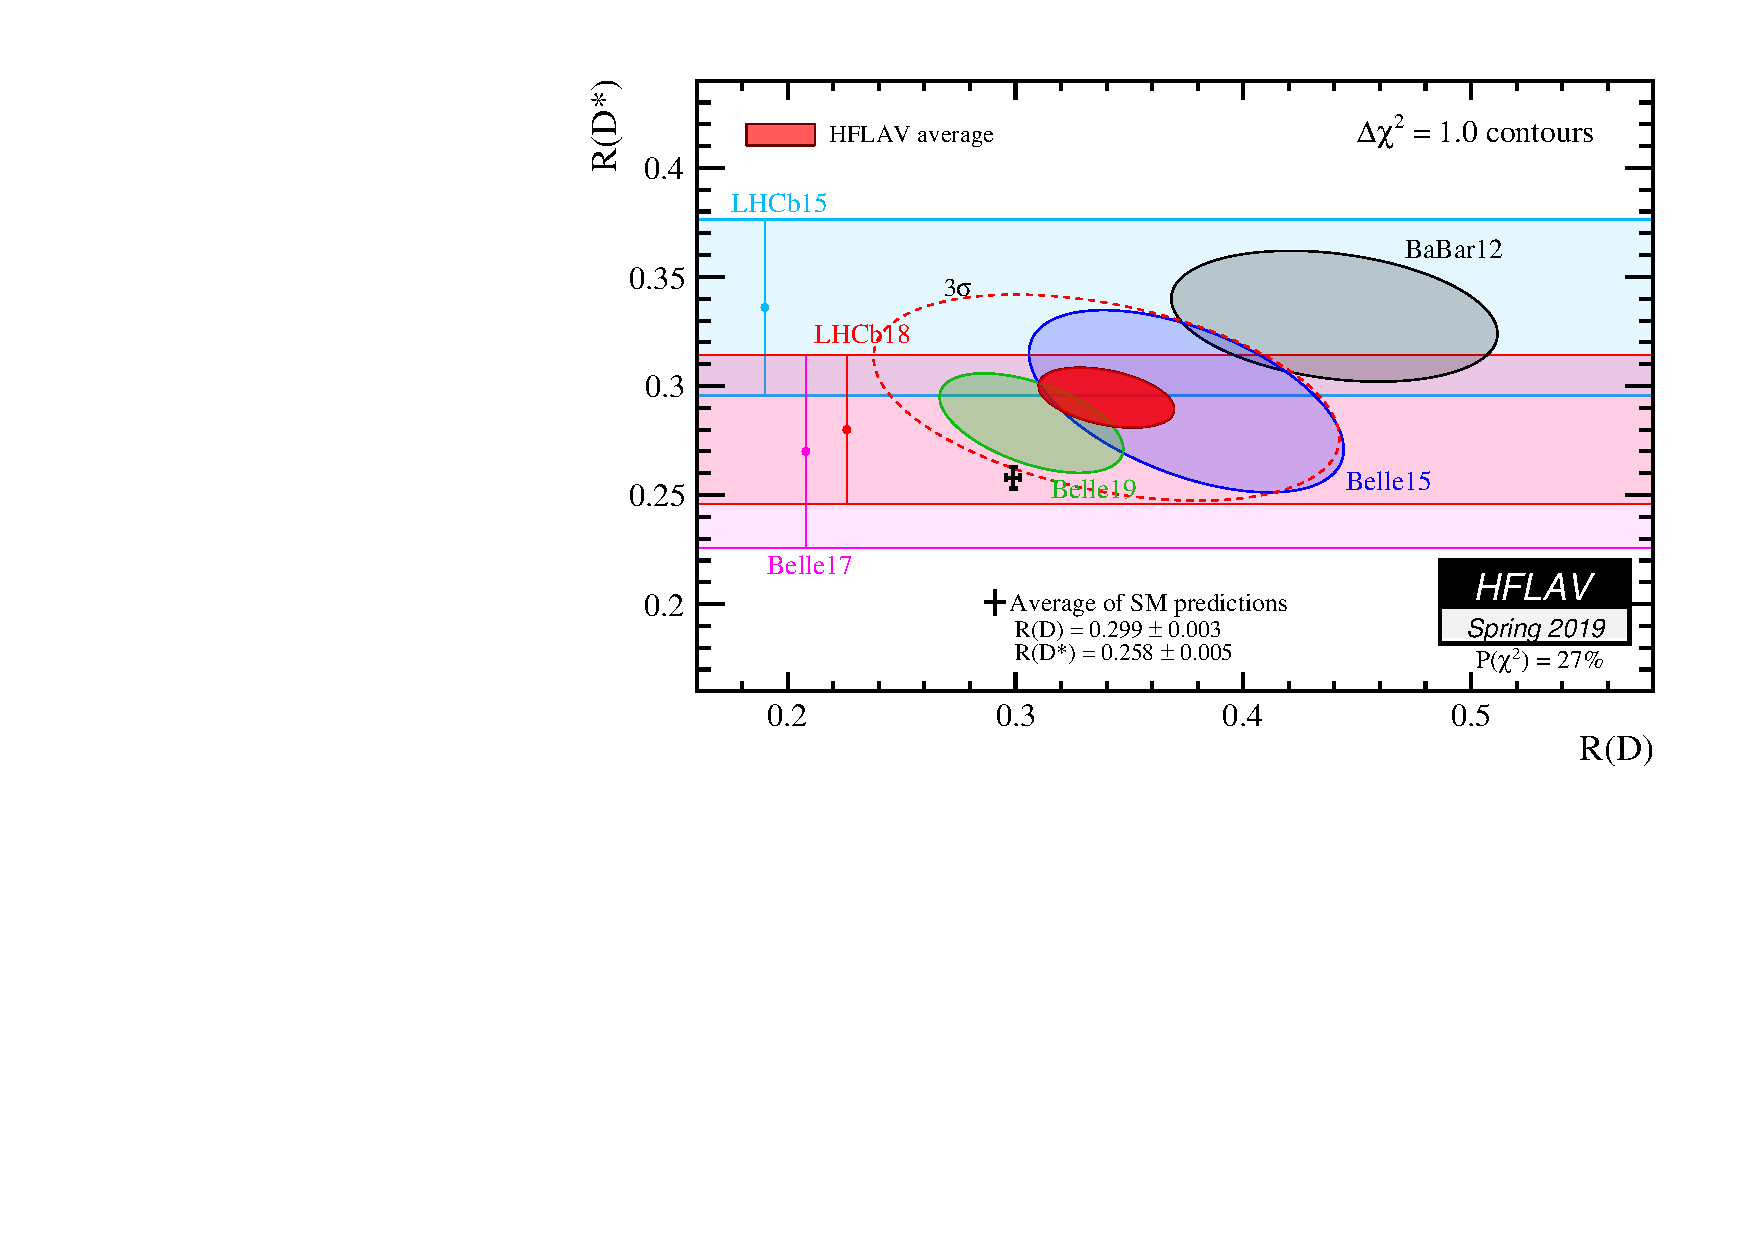
\includegraphics[height=9cm]{fig/hflav.pdf}
    \end{minipage}
    \begin{minipage}{10cm}
       \subsection*{Abbreviations used above}
       \begin{itemize}
          \item BDT: Boosted Decision Tree
          \item (Ext.) ML: (Extended) Maximum likelihood
          \item Sim. fit: Simultaneous fit
          \item SL: Semileptonic
         \end{itemize}
         \subsection*{Variables}
         \begin{itemize}
            \item $\costhyl = \frac{2 E_\text{beam} E_{D^{(*)}\ell} - m_B^2 - m_{D^{(*)}\ell}^2}{2|\vec p_B||\vec p_{D^{(*)}\ell}|}$
            \item $q^2=(p_B-p_{D^{(*)}})^2$ Hadronic recoil
            \item $\mtmiss$: 
               B-factories had. tag $(p_{e^+e^-}-p_\text{tag}-p_{D^{(*)}}-p_\ell)^2$, 
               B-factories SL tag: $(E_{e^+e^-}-\sum_i E_i)^2 - |\sum_i \vec p_i|^2$
               LHCb: $(p_B-p_{D^{(*)}}-p_\mu)^2$ (approximated $p_B$)
            \item $\EECL$ (B-factories): Sum of energy in ECL clusters not used in reconstruction (modulo some subtleties)
            \item $\Evis$ (B-factories): Sum of all energies of reconstructed particles
         \end{itemize}
    \end{minipage}
\end{document}
